\chapter{Grundlagen}
\label{chap:basics}

Im folgenden Kapitel werden die Techniken erläutert, die als Grundlage für diese Diplomarbeit dienen. Im Abschnitt über Themenmodelle wird hergeleitet, wie aus einem Korpus von Dokumenten ein Themenmodell erzeugt. Dabei wird insbesondere auf die statistische Inferenz eingegangen. Im Abschnitt über Zentralitäten werden die benutzten Zentralitätsindizes erläutert.

Es wird folgende Notation durchgängig zur Bezeichnung von Wörtern, Dokumenten und Korpora benutzt\footnote{Die Notation und die folgende Herleitung wurde zu Teilen aus \citep{parameterEstimation} übernommen}.
\begin{itemize}
  \item Ein Korpus $\mathcal{W}=(\doc_1,\ldots,\doc_M)$ besteht aus $M$ Dokumenten. 
  \item Jedes Dokument $\doc_m=(\word_{m,1},\ldots,\word_{m,N})$ besteht aus einer Sequenz von $N$ Wörtern $\word_{m,n}$. Mit $n = \left\lbrace 1,\ldots,N\right\rbrace$ und $m = \left\lbrace 1,\ldots,M\right\rbrace$. 
  \item Ein Wort $\word_{m,n}$ bezeichnet das $n$-te Wort in Dokument $\doc_m$. Ein Wort ist ein Vorkommen eines Terms $t$ aus dem Vokabular $V$. Mehrere Wörter können den gleichen Term instantiieren. So enthält der Satz \textit{Ein Affe bleibt ein Affe, auch in Seide gekleidet} zweimal das Wort \textit{Affe}, dieses instantiiert aber denselben Term \textit{Affe}. 
  \item Ein Term $t$ ist ein eindeutiges Merkmal im zugrundeliegenden Korpus. Im vorliegenden Fall sind dies Wörter im herkömmlichen Sinne. So ist z. B. \textit{Affe} ein Term während \textit{Affen} ein anderer Term ist. 
  \item Mit $\wordTopic_{m,n}$ wird das zugehörige Thema des Wortes $\word_{m,n}$ in Dokument $\doc_m$ bezeichnet. Ein Thema ist hier keine semantische Einheit im klassischen Sinne. Wie ein Thema definiert ist wird im folgenden Abschnitt \ref{sec:topicModels} erklärt.
  \item $\docTopic_m$ bezeichnet die Themen des Dokumentes $\doc_m$. Es ist $\docTopic_m =$\\ $\left(\wordTopic_{m,1},\ldots,\wordTopic_{m,N}\right)$
\end{itemize}

\section{Themenmodelle}
\label{sec:topicModels}

Ein Themenmodell \citep{Hofmann1999,Blei2003LDA,Steyvers2006} ist ein statistisches Modell um Themen aus Textkorpora zu extrahieren. Dazu werden Terme gruppiert, die oft zusammen auftreten. Diese Gruppierung wird als Thema bezeichnet. Ein Thema ist demnach durch die Verteilung der zugehörigen Terme charakterisiert. Ein Term kann dabei zu mehreren Themen gehören. 

Die  Themen werden mit den zwei Termen, die mit der höchsten Wahrscheinlichkeit zu einem Thema gehören, benannt. Die beiden Themen in Abbildung \ref{fig:tmGenerator} würden mit \textit{film regisseur} und \textit{erdbeben richterskale} bezeichnet. So kann in mehr oder weniger direkt auf den Inhalt des Themas geschlossen werden und die Themenbezeichnung ist besser lesbar.  

Um die Themen aus dem Textkorpus zu extrahieren, wird ausgehend von einem generativen Modell eine Methode zur Inferenz der Themen aus den beobachteten Wörtern entwickelt. 
\begin{figure}[ht]
  \centering
  \subfigure[Generativer Prozess]{
    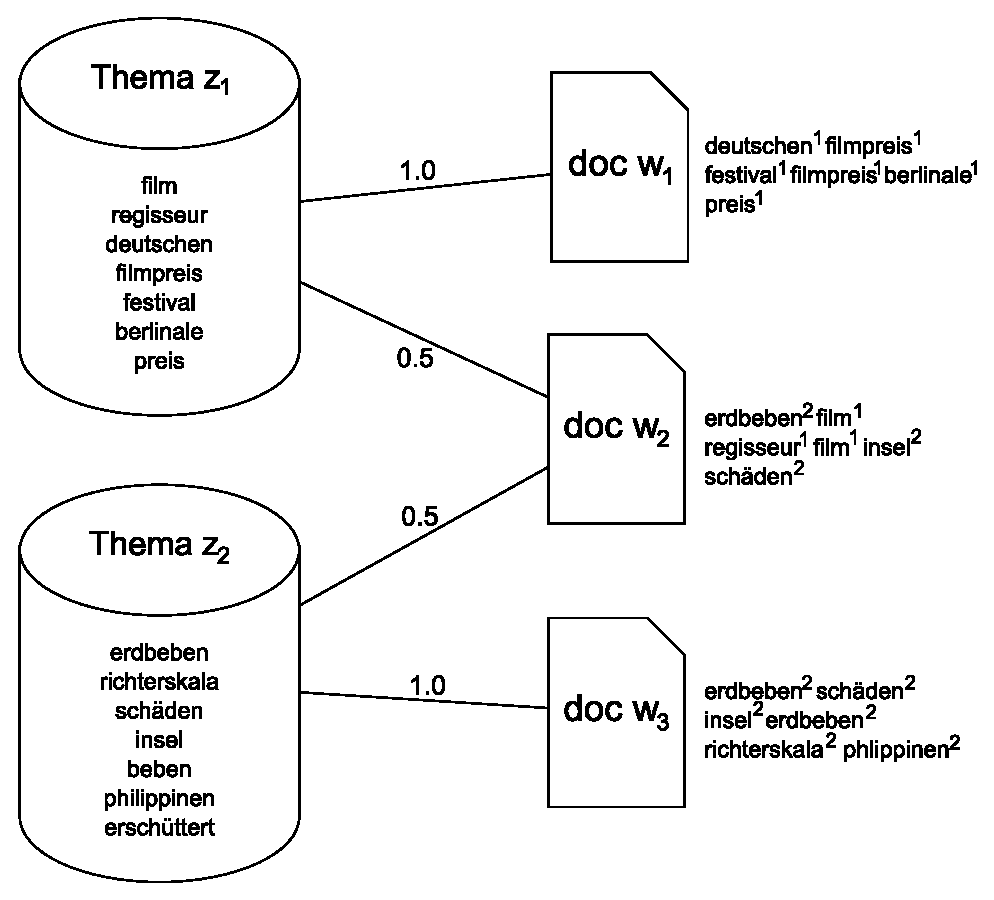
\includegraphics[scale=0.4]{images/content/02_fundamentals/topicModelGenerater}
    \label{fig:tmGenerator}
  }
  \subfigure[Statistische Inferenz]{
    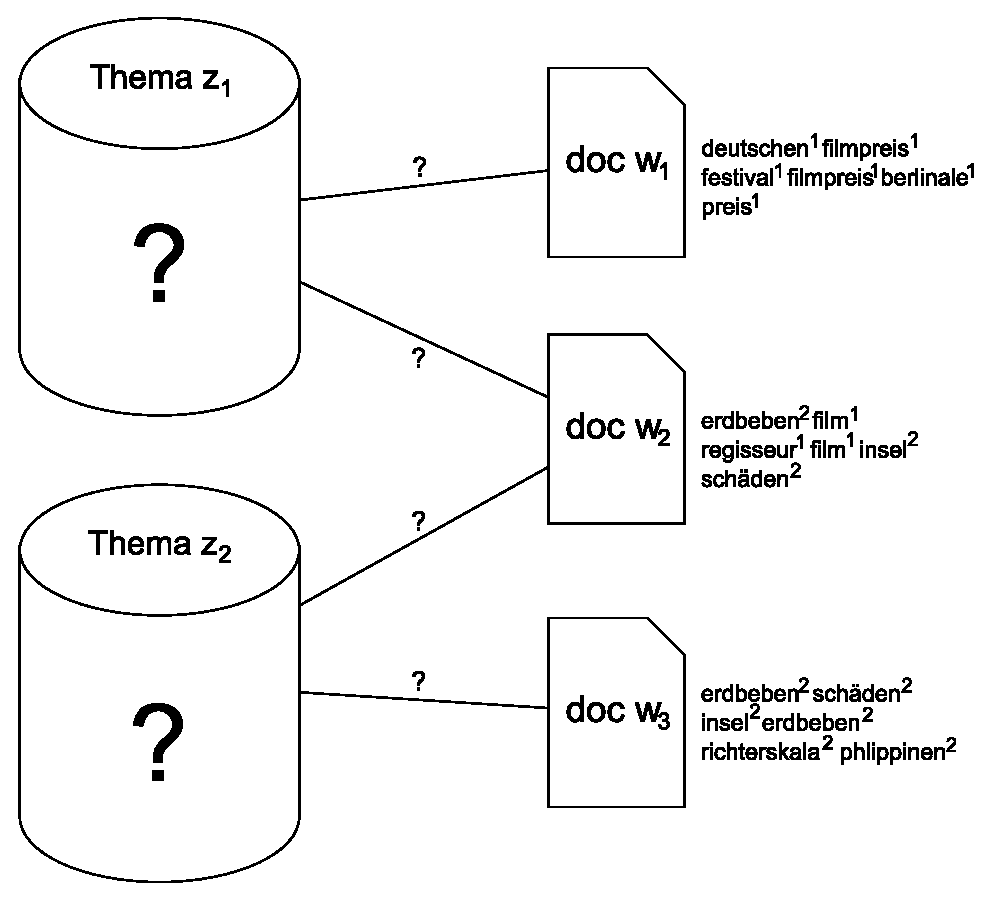
\includegraphics[scale=0.4]{images/content/02_fundamentals/topicModelStatInf}
    \label{fig:tmStatInf}
  }
\caption{Problemstellung der Themen Modelle nach \citep{Steyvers2006}.}
\end{figure}

Der generative Prozess beschreibt, wie aus Themen und den zugehörigen Termen Dokumente generiert werden. Dazu fassen Themenmodelle die Dokumente als Mischung verschiedener Themen auf. Für jedes Dokument wird eine Wahrscheinlichkeit festgelegt, mit der dieses Dokument zu einem Thema gehört. Anhand dieser Wahrscheinlichkeit wird für jedes Wort in einem Dokument ein Term aus dem Thema gezogen. In Abbildung \ref{fig:tmGenerator} wird dieser Prozess schematisch dargestellt. 

Hier werden zwei Themen dargestellt, einmal ein Thema über Filme und ein Thema über Erdbeben. Für Dokument $\doc_1$ und $\doc_3$ wurde jeweils festgelegt, dass sie nur aus Thema $\docTopic_1$ bzw. $\docTopic_2$ bestehen. Dementsprechend werden Wörter nur aus den Termen des zugehörigen Themas gezogen. Dokument $\doc_2$ besteht jeweils zur Hälfte aus Thema $\docTopic_1$ und $\docTopic_2$. Es werden also Terme aus beiden Themen gezogen. Für jedes Wort wird vorher ermittelt, aus welchem Thema ein Term gezogen werden soll. Anschließend wird aus dem so bestimmten Thema ein Term gezogen. So kann ein Dokument generiert werden, das sowohl das Thema Film als auch Erdbeben beinhaltet. Die so generierten Dokumente weisen keine syntaktische Struktur auf, da vom generativen Prozess keine vollständigen Sätze erzeugt werden. Die Wörter instantiieren nur Terme aus den Themen. Dafür sind die Wahrscheinlichkeiten der Themen in diesem Dokument bekannt.

Das generative Modell erlaubt es zwar Dokumente zu bestimmten Themen zu erzeugen, die eigentliche Zielsetzung ist jedoch, für ein Textkorpus Themen zu identifizieren. Die Abbildung \ref{fig:tmStatInf} zeigt analog zu Abbildung \ref{fig:tmGenerator} das Problem auf: Aus Wörtern, die in Dokumenten beobachtet wurden, sollen Themen abgeleitet werden. 
Aus dem generativen Modell kann man mit statistischen Mitteln eine Methode entwickeln, die es erlaubt, aus den beobachteten Daten das dazu passende Modell zu finden. Im folgenden wird anhand der Latent Dirichlet Allocation (LDA) diese Methode hergeleitet. 

\subsection{Latent Dirichlet Allocation}

Der Algorithmus Latent Dirichlet Allocation (LDA) gibt ein probabilistisches Modell zur Erzeugung von Dokumenten an. Anhand dieses Modells kann eine Methode zur statistischen Inferenz von Themen aus beobachteten Wörtern entwickelt werden. In Abbildung \ref{fig:ldaModel} wird das generative Modell als graphisch dargestellt. Im Unterschied zu anderen Themenmodellen gibt die LDA zusätzlich zur Termverteilung von Themen noch eine Themenverteilung für Dokumente an \citep{Hofmann1999}. 

\begin{figure}[ht]
  \centering
  \begin{pspicture}(0,-0.5)(4,6)

\pscircle[fillstyle=solid, fillcolor=grey](2,1){0.5} 
\rput(1.1,1){$w_{m,n}$}
\pscircle(2,3){0.5} 
\rput(1.1,3){$z_{m,n}$}
\pscircle(2,5){0.5} 
\rput(1.1,5){$\vartheta_{m}$}
\psline{<-}(2,1.5)(2,2.5)
\psline{<-}(2,3.5)(2,4.5)

\pscircle(4.5,5){0.5}
\psline{<-}(2.5,5)(4,5)
\rput(4.5,4.25){$\alpha$}

\pscircle(4.5,1){0.5}
\psline{<-}(2.5,1)(4,1)
\rput(4.5,1.75){$\varphi_{k}$}

\pscircle(6.5,1){0.5}
\psline{<-}(5,1)(6,1)
\rput(6.5,1.75){$\beta$}

\psframe(0.2,-0.5)(3.5,6)
\rput(3.2,-0.2){$M$}

\psframe(0.6,0.3)(3.2,4.0)
\rput(2.9,0.6){$N$}

\psframe(3.75,0.25)(5.5,2.0)
\rput(5.2,0.5){$K$}

\end{pspicture}
  \caption{Generatives Modell für LDA nach \citep{Blei2003LDA}.}
  \label{fig:ldaModel}
\end{figure}

In Abbildung \ref{fig:ldaModel} wird dargestellt, wie ein Dokument erzeugt wird. Die Pfeile geben Abhängig"-keiten zwischen den Variablen an, während die Kacheln Wiederholungen von Variablen anzeigen. Die Buchstaben in den Kacheln geben an, wie oft die Variablen wiederholt werden. So können die Knoten für $M$ Dokumente und $M \times N$ Wörter präziser dargestellt werden ohne die Variablen mehrfach zu notieren. Der schattierte Knoten gibt an, dass diese Variable beobachtbar ist und die leeren Knoten zeigen latente Variablen an. 

Für jedes Dokument $\doc_m$, wird eine Themenverteilung $\docTopicDist{m}$ ermittelt. Anhand dieser wird für jedes Wort $\word_{m,n}$ aus Dokument $\doc_m$ ein Thema $\wordTopic_{m,n}=k$ gezogen. Aus der Termverteilung $\topicTermDist{k}$ für das Thema $\wordTopic_{m,n}=k$ wird nun der Term bestimmt, der das Wort instantiiert. 

Die Parameter $\alpha$ und $\beta$ sind die Parameter der Dirichletverteilung, anhand derer die multinomialen Themenverteilungen $\docTopicDist{m}$ und die Termverteilungen $\topicTermDist{k}$ bestimmt werden. Im Weiteren wird $\alpha$ bzw. $\beta$ synonym für $\alpha := (\alpha_1,\ldots,\alpha_k)$ und die symmetrische Variante $\alpha := \alpha_1 = \ldots = \alpha_k$ benutzt. Die Menge aller Themenverteilungen $\docTopicDist{m}$ wird als $\Theta = \left\{\docTopicDist{m}\right\}^M_{m=1}$ bezeichnet und die Menge aller Wortverteilungen $\topicTermDist{k}$ als $\Phi = \left\{\topicTermDist{k}\right\}^K_{k=1}$. 

Aus dem generativen Modell können nun verschiedene Wahrscheinlichkeiten abgeleitet werden. So ist die Wahrscheinlichkeit, dass ein Wort $w_{m,n}$ einen Term $t$ instantiiert, gegeben eine Themenverteilung $\docTopicDist{m}$ für das Dokument $m$
\begin{equation}
  p(\word_{m,n}=t|\docTopicDist{m},\Phi) = \sum^K_{k=1} p(\word_{m,n}=t|\topicTermDist{k})p(\wordTopic_{m,n}=k|  \docTopicDist{m})
\label{eq:ldaWordProbabilty}
\end{equation}
Dies entspricht einer Iteration der Wortkachel, die die Knoten $\wordTopic_{m,n}$ und $word_{m,n}$ enthält. Die gemeinsame Wahrscheinlichkeitsverteilung für alle beobachteten und unbeobachteten Variablen kann anhand des Modells in Abbildung \ref{fig:ldaModel} abgeleitet werden. 
\begin{equation}
p(\doc_m,\docTopic_m,\docTopicDist{m},\Phi|\alpha,\beta) = \overbrace{\underbrace{\prod^{N_m}_{n=1}p(w_{m,n}|\topicTermDist{\wordTopic_{m,n}})p(\wordTopic_{m,n}|\docTopicDist{m})}_{\text{Wortkachel}} \cdot p(\docTopicDist{m}|\alpha)}^{\text{Dokumentkachel (nur 1 Dokument)}} \cdot \underbrace{p(\Phi|\beta)}_{\text{Themenkachel}}
\label{eq:ldaDocJointDistribution}
\end{equation}

Integriert man nun über $\docTopicDist{m}$ und $\Phi$ und summiert über alle Themen $\wordTopic_{m,n}$ erhält man mit (\ref{eq:ldaWordProbabilty}), die Wahrscheinlichkeit für ein Dokument $\doc_m$.

\begin{align}
p(\doc_m|\alpha,\beta) &= \int \int p(\docTopicDist{m}|\alpha)p(\Phi|\beta)\cdot \prod^{N_m}_{n=1} \sum_{\wordTopic_{m,n}} p(\word_{m,n}|\topicTermDist{\wordTopic_{m,n}})p(\wordTopic_{m,n}|\docTopicDist{m})d\Phi d\docTopicDist{m} \\ &=  \int \int p(\docTopicDist{m}|\alpha)p(\Phi|\beta)\cdot \prod^{N_m}_{n=1} p(\word_{m,n}|\docTopicDist{m},\Phi)d\Phi d\docTopicDist{m}
\label{eq:ldaDocDistribution} 
\end{align}

Die Wahrscheinlichkeit für ein komplettes Korpus erhält man, indem man $M$ mal ein Dokument erzeugt. Die Wahrscheinlichkeit für ein Korpus kann also mit folgender Formel ausgedrückt werden.

\begin{equation}
p(\corpus|\alpha,\beta) = \prod^M_{m=1} p(\doc_m|\alpha,\beta)
\end{equation}

\subsection{Inferenz mit Gibbs-Sampling}

Man kann nun ausgehend von diesen Wahrscheinlichkeiten eine Methode zur Inferenz der unbeobachteten Themen entwickeln. Hierzu nutzt man einen approximativen Algorithmus, da trotz der relativen Einfachheit des Modells eine exakte Inferenz nicht möglich ist. Hier benutzen wir dazu Gibbs-Sampling \citep{Walsh2004} . 

Gibbs-Sampling ist eine Monte Carlo Markov Ketten (MCMC) Simulation. Mit MCMC Methoden kann man hochdimensionale  Wahrscheinlichkeitsverteilungen anhand einer Markov Kette simulieren. Dies erlaubt es, die gesuchte Verteilung $p(\docTopic|\doc)$, welche Themen in welchen Dokumenten auftreten, zu berechnen. Mit exakter Inferenz ist diese Verteilung sehr schwierig zu berechnen \citep{parameterEstimation}. Der Gibbs-Sampling Algorithmus berechnet die Verteilung nicht exakt sondern nähert die Verteilung an. Der Algorithmus funktioniert wie folgt.

Sei $p(w,z)$ eine bivariate Zufallsvariable. Wir wollen $p(z)$ bzw. $p(w)$ berechnen. Anstatt nun $\int p(w,z)dw$ bzw. $\int p(w,z)dz$ direkt zu berechnen, berechnet der Gibbs-Sampler alternierende Sequenzen von $p(w|z)$ und $p(z|w)$. Das Sampling wird mit einem zufälligen Wert für $z_0$ gestartet und sampelt $w_0$ anhand $p(w|z=z_0)$. Dann wird $w_0$ dazu benutzt $z_1$ anhand der bedingten Verteilung $p(z|w=w_0)$ zu ermitteln. Das Sampling wird dann nach folgender Formel fortgesetzt:
\begin{align*}
w_i & \approx p(w|z=z_{i-1})  \\
z_i & \approx p(z|w=w_{i})
\end{align*}
Nach $k$-maliger Wiederholung konvergiert die Sequenz gegen die tatsächliche Verteilung. 

Für den multivariaten Fall wird die bedingte Wahrscheinlichkeit erweitert, indem aus dem Variablenvektor $\mathbf{w}$ die $k$-te Variable aus der Verteilung $p(w_i|\mathbf{w}_{\neg i})$ gezogen wird. Wobei $\mathbf{w}_{\neg i} = (w_1,\ldots,w_{i-1},w_{i+1},\ldots,w_k)$ ist. 

Für die LDA wollen wir nun die Verteilung $p(\docTopic|\doc)$ abschätzen. Um dies berechnen zu können, müssen wir die gemeinsame Verteilung $p(\docTopic,\doc)$ bzw. $p(\doc)$ kennen (siehe Gleichung \ref{eq:gibbsLDA})

\begin{align}
p(\docTopic|\doc) = \frac{p(\doc,\docTopic)}{p(\doc)} = \frac{\prod^W_{i=1}p(\word_i|\wordTopic_i)}{\prod^W_{i=1}\sum^K_{k=1}p(\wordTopic_i=k,\word_i)}
\label{eq:gibbsLDA}
\end{align}

Hier hilft uns die Gibbs-Sampling Prozedur, die es erlaubt, $p(\docTopic|\doc)$ direkt zu berechnen, ohne über $K^W$ Terme zu summieren. Der Gibbs-Sampler simuliert die Verteilung $p(\docTopic|\doc)$ durch 
\begin{equation}
p(\wordTopic_i|\docTopic_{\neg i }, \doc) = \frac{p(\doc,\docTopic)}{p(\docTopic_{\neg i},\doc)} 
\end{equation}

Hierzu müssen wir die gemeinsame Verteilung $p(\doc,\docTopic)$ kennen. Im Falle der LDA kann diese Verteilung aufgespalten werden in 
\begin{equation}
p(\doc,\docTopic|\alpha,\beta) = p(\doc|\docTopic,\beta)\cdot p(\docTopic|\alpha)\text{,}
\end{equation}
da $\doc$ unabhängig von $\alpha$ ist und $\docTopic$ unabhängig von $\beta$.

Die Faktoren können einzeln hergeleitet werden. So ist 
\begin{align}
p(\doc|\docTopic,\beta) &= \int p(\doc|\docTopic,\Phi) p(\Phi|\beta) d\Phi \notag \\
                        &= \int \prod^K_{z=1}\frac{1}{\Delta(\beta)} \prod^V_{t=1}\topicTermProb{z}{t}^{n^{(t)}_z+\beta_t-1} d\topicTermDist{z} \label{eq:ldaGibbsIntegral1}\\
                        &= \prod^K_{z=1}\frac{\Delta(\mathbf{n}_z+\beta)}{\Delta(\beta)}, \ \ \mathbf{n}_z=\left\lbrace n_z^{(t)}\right\rbrace^V_{t=1} \label{eq:ldaGibbsIntegral2}
\end{align}

Hier wird benutzt, dass $p(\doc|\docTopic,\Phi)$ multinomial und $p(\Phi|\beta)$ dirichlet verteilt ist. Unter der Annahme, dass die Reihenfolge der Wörter in einem Dokument unerheblich ist, gilt:
\begin{align*}
p(\doc|\docTopic,\Phi) %&= \prod^W_{i=1}p(\word_i|\wordTopic_i) = \prod^W_{i=1}\topicTermProb{z_i}{w_i} \\
					   &= \prod^K_{k=1}\prod_{i:z_i=k}p(\word_i=t|\wordTopic_i=k) = \prod^K_{k=1}\prod^V_{t=1}\topicTermProb{k}{t}^{n^{(t)}_k}
\end{align*}
und 
\begin{align*}
Dir(\topicTermDist{k}|\beta) = \frac{1}{\Delta(\beta)}\prod^V_{t=1} \topicTermProb{k}{t}^{\beta_{t}-1} \text{ mit } \Delta(\beta)=\frac{\prod^{dim \beta}_{k=1}\Gamma(\beta_k)}{\Gamma(\sum^{dim \beta}_{k=1}\beta_k)}
\end{align*}
Aus den beiden vorhergehenden Gleichungen ergibt sich \ref{eq:ldaGibbsIntegral1}. Die Anwendung des Dirichletintegrals auf Gleichung \ref{eq:ldaGibbsIntegral1} ergibt dann Gleichung \ref{eq:ldaGibbsIntegral2}.

Analog kann $p(\docTopic|\beta)$ hergeleitet werden. Es ist:
\begin{align}
p(\docTopic|\alpha) &= \int p(\docTopic|\Theta) p(\Theta|\alpha) d\Theta \notag\\
                    &= \int \prod^M_{m=1}\frac{1}{\Delta(\alpha)}\prod^K_{k=1}\docTopicProb{m}{k}^{n^{(k)}_m + \alpha_k-1}  d\docTopicDist{m} \\
                    &= \prod^M_{m=1} \frac{\Delta(\mathbf{n}_m+\alpha)}{\Delta(\alpha)}, \ \ \mathbf{n}_m=\left\lbrace n_m^{(k)}\right\rbrace^K_{k=1} \label{eq:ldaPZ}
\end{align}

Die gemeinsame Verteilung $p(\doc,\docTopic|\alpha,\beta)$ ergibt sich aus \ref{eq:ldaPZ} und \ref{eq:ldaGibbsIntegral2}. 
\[
p(\doc,\docTopic|\alpha,\beta) = \prod^K_{z=1}\frac{\Delta(\mathbf{n}_z+\beta)}{\Delta(\beta)} \cdot \prod^M_{m=1} \frac{\Delta(\mathbf{n}_m+\alpha)}{\Delta(\alpha)}
\]

Wenn man nun die gemeinsame Verteilung einsetzt, ergibt sich die Update-Gleichung für den Gibbs-Sampler. 

\begin{align}
p(\wordTopic_i=k|\docTopic_{\neg i},\doc) &= \frac{p(\doc,\docTopic)}{p(\doc,\docTopic_{\neg i})} = \frac{p(\doc,\docTopic)}{p(\doc_{\neg i},\docTopic_{\neg i})p(\word_i)} \frac{p(\docTopic)}{p(\docTopic_{\neg i})} \\
&\propto \frac{\Delta(\mathbf{n}_z+\beta)}{\Delta(\mathbf{n}_{z,\neg i} + \beta)} \cdot \frac{\Delta(\mathbf{n}_m+\alpha)}{\Delta(\mathbf{n}_{m.\neg i} + \alpha)} \\
&\propto \ldots \notag \\
&\propto \frac{n^{(t)}_{k,\neg i}+\beta}{\sum^{V}_{t=1}n^{(t)}_{k,\neg i} + \beta} \cdot \frac{n^{(k)}_{m,\neg i}+\alpha}{\sum^{K}_{k=1}n^{(k)}_{m,\neg i} + \alpha} \label{eq:updateEqSeen}
\end{align} 

Die Update-Gleichung kann nun dazu benutzt werden, die Themen für Wörter in Dokumenten zu bestimmen. Es wird über alle Wörter in den Dokumenten iteriert und für jedes Wort anhand $p(\wordTopic_i=k|\docTopic_{\neg i},\doc)$ ein neues Thema bestimmt. Dies wird solange wiederholt, bis die Themenverteilung stabil bleibt, bzw. der Gibbs-Sampler einen stabilen Zustand erreicht hat. Die Verteilungen $\docTopicDist{m}$ und $\topicTermDist{k}$ können direkt aus den Gleichungen \ref{eq:ldaGibbsIntegral2} und \ref{eq:ldaPZ} abgeleitet werden. So hat man nun ein Modell, welches Dokumente bzw. Wörter in Themen gruppieren kann. Genaueres zur Herleitung und Gibbs-Sampling im Kontext der LDA kann in \citep{Griffiths2004LDA} nachgelesen werden.

\subsection{Inferenz für ungesehene Dokumente}
\label{subsec:infUnseen}

Ausgehend vom gelernten Modell will man nun für neue Dokumente die Themen herausfinden. Sei $\tilde{\doc}$ ein neues Dokument. Für dieses neue Dokument lassen wir wiederum den Gibbs-Sampler die Themen bestimmen. Anstatt $p(\wordTopic_i=k|\docTopic_{\neg i},\doc)$ bestimmen wir aber $p(\tilde{\wordTopic}_i=k|\tilde{\docTopic}_{\neg i},\tilde{\doc},\Phi,\Theta)$, da wir die Themen für das neue Dokument anhand der schon ermittelten Themen- und Termverteilungen inferieren wollen. Es ergibt sich folgende Update-Gleichung
\begin{equation}
p(\tilde{\wordTopic}_i=k|\tilde{\docTopic}_{\neg i},\tilde{\doc},\Phi,\Theta) = \frac{n^{(t)}_{k}+\tilde{n}^{(t)}_{k, \neg i}+\beta}{\sum^V_{t=1}n^{(t)}_{k}+\tilde{n}^{(t)}_{k, \neg i}+\beta}\cdot \frac{n^{(k)}_{\tilde{m},\neg i}+\alpha}{\sum^K_{k=1}n^{(k)}_{\tilde{m},\neg i}+\alpha} 
\label{eq:updateEqUnseen}
\end{equation}
wobei $\tilde{n}^{(t)}_{k}$ die Anzahl des Auftreten von Term $t$ mit Thema $k$ für das neue Dokument $\tilde{\doc}$ bezeichnet. Analog zu normaler Inferenz können auch hier die Dokumentverteilung $\docTopicDist{m}$ und die Termverteilung $\topicTermDist{k}$ bestimmt werden. So können für ein neues Dokument die vorherrschenden Themen bestimmt werden. 

Ein Problem sind Terme, die vorher nicht aufgetreten sind. Diese erscheinen in den Termverteilungen der Themen nicht und können somit nicht dazu beitragen, Themen zu inferieren. Sie fließen somit auch nicht in die Updategleichung \ref{eq:updateEqUnseen} mit ein. Im Falle der Inferenz werden sie einfach übersprungen.



\section{Zentralitätsindizes}
\label{sec:centralities}

Ein Zentralitätsindex ist ein Maß, das intuitiv die Wichtigkeit eines Knoten oder einer Kante in einem Graphen wiedergibt. Betrachtet man den Graphen in Abbildung \ref{fig:randomGraph} als Straßennetzwerk, welches verschiedene Knotenpunkte miteinander verbindet und möchte herausfinden, welcher Knotenpunkt der am meisten belastete ist, kann dies durch ein Zentralitätsmaß erfasst werden. Ein Zentralitätsmaß weist jedem Knoten einen Wert zu, der die Wichtigkeit dieses Knoten widerspiegelt. So ist in der Abbildung der Knoten $F$ augenscheinlich der Knoten, der am meisten belastet wird. Zählt man nun für jeden Knoten die Anzahl der Kanten und benutzt den ermittelten Wert als Zentralitätsmaß, ergeben sich die Zentralitätswerte in Abbildung \ref{fig:randomGraphCentrality}. Das Zentralitätsmaß gibt das Erwartete wieder, da dem Knoten $F$ der größte Wert (5) zugewiesen wird. 

\begin{figure}[ht]
\centering
  \subfigure[Straßennetzwerk]{
    \begin{pspicture}(0,0)(5,4)

\cnode[fillstyle=solid, fillcolor=white](0,1){0.3}{B}
\cnode[fillstyle=solid, fillcolor=white](0,2.5){0.3}{A}

\cnode[fillstyle=solid, fillcolor=white](1,1){0.3}{E}
\cnode[fillstyle=solid, fillcolor=white](1,2){0.3}{D}
\cnode[fillstyle=solid, fillcolor=white](1,3){0.3}{C}

\cnode[fillstyle=solid, fillcolor=grey](2.5,2){0.3}{F}

\cnode[fillstyle=solid, fillcolor=white](4,1){0.3}{H}
\cnode[fillstyle=solid, fillcolor=white](4,3){0.3}{G}

\ncline{A}{C}
\ncline{A}{D}
\ncline{B}{E}

\ncline{C}{F}
\ncarc{C}{G}
\ncline{D}{F}
\ncline{E}{F}

\ncline{F}{H}
\ncline{F}{G}

\rput(0,1){$B$}
\rput(0,2.5){$A$}

\rput(1,1){$E$}
\rput(1,2){$D$}
\rput(1,3){$C$}

\rput(2.5,2){$F$}

\rput(4,1){$H$}
\rput(4,3){$G$}

\end{pspicture}

    \label{fig:randomGraph}
  }
  \subfigure[Straßennetzwerk mit Zentralitäten]{
    \begin{pspicture}(0,0)(5,4)

\cnode[fillstyle=solid, fillcolor=white](0,1){0.3}{B}
\cnode[fillstyle=solid, fillcolor=white](0,2.5){0.3}{A}

\cnode[fillstyle=solid, fillcolor=white](1,1){0.3}{E}
\cnode[fillstyle=solid, fillcolor=white](1,2){0.3}{D}
\cnode[fillstyle=solid, fillcolor=white](1,3){0.3}{C}

\cnode[fillstyle=solid, fillcolor=grey](2.5,2){0.3}{F}

\cnode[fillstyle=solid, fillcolor=white](4,1){0.3}{H}
\cnode[fillstyle=solid, fillcolor=white](4,3){0.3}{G}

\ncline{A}{C}
\ncline{A}{D}
\ncline{B}{E}

\ncline{C}{F}
\ncarc{C}{G}
\ncline{D}{F}
\ncline{E}{F}

\ncline{F}{H}
\ncline{F}{G}

\rput(0,1){1}
\rput(0,2.5){2}

\rput(1,1){2}
\rput(1,2){2}
\rput(1,3){3}

\rput(2.5,2){5}

\rput(4,1){1}
\rput(4,3){2}

\end{pspicture}

    \label{fig:randomGraphCentrality}
  }

\caption{Zentralitäten in einem Graphen}
\end{figure}

Es gibt noch viele anderen Zentralitätsmaße, die verschiedene Aspekte betrachten. Im Folgenden werden einige der für die Arbeit geeignet erscheinenden Zentralitätsmaße definiert und untersucht. Dazu benötigen wir zunächst einige wichtige Definitionen aus der Graphentheorie. 

\paragraph{Definition:} Ein Graph $G$ ist ein Tripel $(V,E,\omega)$, wobei $V=\lbrace v_1,\ldots,v_n\rbrace$ eine Menge von Knoten ist, $E=\lbrace e_1,\ldots,e_m \rbrace$ eine Menge von Kanten und $\omega: E \rightarrow \mathbb{R}$ eine Funktion, die jeder Kante $e \in E$ eine reelle Zahl zuordnet. 

Es kann zwischen gerichteten Graphen und ungerichteten Graphen unterschieden werden. Im ungerichteten Fall gilt
\[
E \subseteq \left\lbrace \{v,u\} | v,u \in V \right\rbrace \text{,}
\]
d.h. die Kante $\lbrace u,v \rbrace$ ist dieselbe wie $\lbrace v,u \rbrace$, da die Kanten als Mengen betrachtet werden und diese nicht sortiert sind. Im gerichteten Fall gilt
\[
E \subseteq \left\lbrace (u,v) | u,v \in V\right\rbrace \text{,}
\]
hier wird zwischen $(u,v) \in E$ und $(v,u) \in E$ unterschieden, da Paare sortiert sind.

Der Grad eines Knoten wird durch die Anzahl der eingehenden Kanten bzw. der ausgehenden Kanten bestimmt. Es ist $o(v)$ die Menge der ausgehenden Kanten eines Knoten $v$. Analog ist $i(v)$ die Menge der eingehenden Kanten. Im ungerichteten Fall gilt $o(v) = i(v)$. 

Ein Pfad $\pi$ ist definiert als eine Folge von Knoten $(v_1,\ldots,v_i,\ldots,v_n)$, wobei für alle $i,j \in \{1,\ldots,n\}$ gilt, dass $v_i \neq v_j$ falls $i \neq j$.

Die Distanz zwischen zwei Knoten $u$,$v$ wird mit $d(u,v)$ bezeichnet. Die Distanz zwischen zwei Knoten wird als die Summe der Gewichte auf dem Pfad von $u$ nach $v$ definiert. Im Falle, dass kein Pfad von $u$ nach $v$ existiert, gilt $d(u,v) = \infty$ und es gilt $d(u,u) = 0$. 

Eine formale Definition für Zentralitätsindizes wurde bis jetzt nicht aufgestellt. In \citet{Brandes2005} wird versucht, eine formalen Definition anzugeben. Dazu wird ein Zentralitätsindex als struktureller Index aufgefasst, der eine Halbordnung auf die Knoten bzw. Kanten des Graphen induziert. 

\paragraph{Definition:} Seien $\graph = (\vertexSet_\graph,\edgeSet_\graph)$ und $H=(\vertexSet_H,\edgeSet_H)$ gewichtete Graphen und $\Phi$ der Isomorphismus zwischen $G$ und $H$. Es bezeichne $X$ die Knotenmenge $\vertexSet_\graph$ bzw. die Kantenmenge $\edgeSet_\graph$. Dann ist $s$ ein struktureller Index genau dann, wenn $\forall x \in X: \graph \simeq H \Rightarrow s_\graph(x) = s_H(\Phi(x))$

Ein Zentralitätsindex muss ein struktureller Index sein, wobei nicht jeder strukturelle Index ein Zentralitätsindex ist. Durch die induzierte Halbordnung können wir Aussagen bzgl. eines Zentralitätsindex $\centrality{X}$ treffen, wie $x \in \vertexSet$ ist mindestens so zentral wie $y \in \vertexSet$ wenn $\centrality{X}(x) \geq \centrality{X}(y)$.

Für die einzelnen Klassen der Zentralitätsindizes wird in \citet{Brandes2005} versucht, eine axiomatische Definition herzuleiten. Diese hier wiederzugeben, würde den Fokus der Diplomarbeit verlassen. 

\subsection{Degree-Zentralität}
\label{subsec:degreecentrality}
Degree-Zentralität ist die einfachste Art der Zentralität. Die Zentralität der einzelnen Knoten wird anhand der Anzahl der ein- und ausgehenden Kanten bestimmt. 
Für gerichtete Graphen kann zwischen eingehenden und ausgehenden Kanten unterschieden werden. So ist die eingehende Degree-Zentralität definiert als \[\centrality{iD}(v) := |i(v)|\] 
und die ausgehende Degree-Zentralität als 
\[\centrality{oD}(v) := |o(v)|\] 
definiert. Im ungerichteten Fall gilt \[\centrality{D}(v) := |o(v)| \mbox{ oder } \centrality{D}(v) := |i(v)| \mbox{.}\]

Ein weiterer Zentralitätsindex bezieht zusätzlich zur Anzahl der Kanten noch die Gewichtung der Kanten mit ein. Die Shaffer-Zentralität $\centrality{SH}$ eines Knoten $v$ ist die Wurzel der Summe der quadrierten Gewichte der ein- bzw. ausgehenden Kanten. 
\[
\centrality{oSH}(v) = \sqrt{\sum_{u \in o(v)} \edgeWeight{(v,u)}^2 } \mbox{ bzw. } \centrality{iSH}(v) = \sqrt{\sum_{u \in i(v)} \edgeWeight{(u,v)}^2 }
\]

Der Vorteil der Degree-Zentralität Indizes ist die Unabhängigkeit von der Struktur des Graphen. Auch wenn der Graph nicht vollständig verbunden ist, können alle Knoten bewertet werden. Dies ist möglich, da die Knoten nur lokal betrachtet werden und die globale Struktur des Graphen außer Acht gelassen wird. Das kann je nach Anwendung ausreichend sein. Betrachtet man jedoch zum Beispiel, das Problem eine industrielle Anlage möglichst nah an allen Zulieferern aufzustellen, muss man die globale Struktur des Graphen berücksichtigen. Dazu eignen sich die folgenden Indizes besser. 

\subsection{Distanz}

Distanzbasierte Zentralitätsindizes berechnen die Zentralität anhand der Distanz zwischen den Knoten im Graphen. Bei distanzbasierten Zentralitäten geht es oft darum, eine öffentliche Einrichtungen in einem bestehenden Straßennetz zu platzieren, so dass bestimmte Kriterien erfüllt sind. 

\subsubsection{Eccentricity-Zentralität}
Ein Anwendungsbeispiel für die Eccentricity-Zentralität ist es, ein Krankenhaus zu platzieren, so dass die maximale Distanz zu allen Haushalten minimiert wird. Hierzu kann man das Exzentrizität-Zentralitätsmaß nutzen. Dieser Index berechnet, inwieweit ein Knoten im ``Inneren'' des Graphen liegt und bestimmt die Zentralität anhand der Exzentrizität der Knoten. Die Exzentrizität $e(v)$ eines Knoten $v$ ist definiert als der längste Pfad zu allen anderen Knoten $u$. D.h. $e(v) := max\lbrace d(u,v) | u \in V\rbrace$. Knoten, die in wenigen Schritten alle anderen Knoten erreichen können und im ``Inneren'' des Graphen liegen, sind somit zentraler als solche die weiter ``außen'' liegen. Die Eccentricity-Zentralität wird als die reziproke Exzentrizität definiert: 
\[\centrality{E}(v) := \frac{1}{e(v)}\]

Die Eccentricity-Zentralität in der obigen Formulierung weist die Schwäche auf, dass sie nur auf ungerichteten und zusammenhängenden Graphen definiert ist. Ist der Graph gerichtet oder nicht zusammenhängend kann es passieren, dass zwei Knoten nicht verbunden sind. Da für zwei Knoten $u,v$, die nicht verbunden sind, gilt, dass $d(v,u) = \infty$, ergibt die Exzentrizität $e(v) = \infty$ für alle Knoten $v$. Daraus folgt, dass die Zentralität $\centrality{E}$ nicht mehr definiert ist.

\subsubsection{Closeness-Zentralität}

Als Beispiel betrachte man das Problem einen Supermarkt zu bauen, so dass die totale Entfernung zu allen möglichen Kunden minimiert wird. Die Closeness-Zentralität kann bei der Lösung dieses Problem helfen. Sie wird als die Summe der Abstände zu allen anderen Knoten des Graphen definiert. Knoten mit einem niedrigen Closeness-Wert sind von allen anderen Knoten leichter erreichbar als Knoten mit einem hohen Wert. Entsprechend sind Knoten mit einem niedrigen Closenesswert zentraler als solche mit hohem Wert. Die Closeness-Zentralität wird dementsprechend analog zur Eccentricity-Zentralität definiert. Als reziproker Wert der Summe aller Pfade von $v$ zu allen anderen Knoten $u$.
\[c_C(v) := \frac{1}{\sum_{u \in V}d(u,v)}\mbox{.}\]
Der Supermarkt muss also an dem Knoten aufgestellt werden, der die höchste Closeness-Zentrali"-tät besitzt.

\subsubsection{Valente-Foreman-Closeness-Zentralität} 

Die Valente-Foreman-Closeness-Zentralität ist ein Abwandlung der Closeness-Zentralität. Sie ist definiert als 
\[
  c_R(v) := \frac{\sum_{u \in V}\Delta_G + 1 - d(v,u)}{n-1}
\] 
wobei $\Delta_G$ der Durchmesser des Graphen (der längste Pfad im Graphen) ist und $n := |V|$. Im Unterschied zur Closeness-Zentralität wird nicht der reziproke Wert der Closeness genommen, sondern die Distanz invertiert und so die entstehenden Werte gemittelt. 

Auch hier gilt, dass die Closeness-Zentralität und die Valente-Foreman-Closeness-Zentralität aus den gleichen Gründen wie die Eccentricity-Zentralität für nicht zusammenhängende oder Spezialfälle von gerichteten Graphen nicht definiert sind.

\subsection{Shortest-Path}

Shortest-Path Zentralitätsindizes für Knoten berechnen die Zentralität anhand der Anzahl der kürzesten Pfade, die durch einen Knoten führen. Betrachtet man wieder ein Straßennetz, in dem die Knoten Mautstationen repräsentieren und möchte wissen, durch welche Mautstation die meisten Fahrzeuge fahren, kann man Shortest-Path-Zentralitäten benutzen. Diese geben wieder, wie viel Arbeit ein Knoten leisten muss, bzw. wie viele Fahrzeuge durch die Mautstation geschleust werden. 

\subsubsection{Stress-Zentralität}

Die Stress-Zentralität misst, wie viel kürzeste Pfade durch einen Knoten im Graphen laufen. Zur Berechnung werden für einen Knoten $v$ die Anzahl der kürzesten Wege, die von einem Knoten $s$ zu einem Knoten $t$ führen, aufsummiert. Die Formel der Zentralität lautet: 
\[c_S(v) := \sum_{s \neq v \in V}\sum_{t \neq v \in V}\sigma_{st}(v)\]
 $\sigma_{st}(v)$ gibt die Anzahl der kürzesten Pfade von $s$ nach $t$ über $v$ an.

Dieser Index funktioniert für gerichtete und ungerichtete Graphen mit Kantengewichten. Definiert man $\sigma_{st}(v) = 0$, wenn es keinen Pfad von $s$ nach $t$ über $v$ gibt, dann funktioniert die Stress-Zentralität auch für nicht zusammenhängende Graphen bzw. für spezielle Konfigurationen von gerichteten Graphen.

\subsubsection{Betweenness -Zentralität}

Betweenness-Zentralität kann als eine Art normalisierte Stress-Zentralität betrachtet werden. Hier wird die Anzahl der kürzesten Pfade von $s$ nach $t$ über $v$ durch die Anzahl aller kürzesten Pfade von $s$ nach $t$ dividiert und somit relativiert. Die Formel ist analog zur Formel der Stress-Zentralität 
\[c_B(v) := \sum_{s \neq v \in V}\sum_{t \neq v \in V}\frac{\sigma_{st}(v)}{\sigma_{st}}\]
Hierbei bezeichnet $\sigma_{st}$ die Anzahl der kürzesten Pfade von $s$ nach $t$. Im Gegensatz zur Stress-Zentralität wird nicht die absolute Anzahl der kürzesten Pfade durch einen Knoten gezählt, sondern die relative Anzahl. So können Knoten, die eine hohe Last haben, besser bewertet werden (siehe \citep{Brandes2005} S. 30 Abb. 3.6).
Im Gegensatz zur Stress-Zentralität funktioniert die Betweenness-Zentralität nicht auf unzusammenhängenden Graphen. Auch hier gilt wieder: Sobald kein Pfad zwischen zwei Knoten $s,t \in \vertexSet$ existiert, ist die Betweenness-Zentralität nicht mehr definiert. 

\subsection{Feedback-Zentralitäten}

Die Feedback Zentralitäten wurden zuerst bei der Bewertung von Webseiten benutzt \citep{pagerank,hits}. Die Idee ist, dass eine Webseite hoch bewertet wird, wenn viele andere gut bewertete Webseiten auf diese verlinken. Die Bewertung bzw. die Zentralität wird an die benachbarten Seiten weitergegeben. So können Seiten, auf die zwar nicht oft verlinkt wird, trotzdem gut bewertet werden, wenn die wenigen verlinkenden Seiten eine hohe Bewertung aufweisen. Zusätzlich werden Seiten mit vielen eingehenden Links besser bewertet. 

\subsubsection{PageRank}
PageRank ist eine solche Feedback-Zentralität \citep{pagerank}. Die Zentralität eines Knoten wird anhand der Zentralitäten der benachbarten Knoten berechnet. Es gilt folgendes zu berechnen. 
\begin{equation}
\centrality{PR}(v) = d \sum_{u \in i(v)}\frac{\centrality{PR}(u)}{|o(u)|} + (1 - d)
\label{eq:prNonRecursiveFromula}
\end{equation}
Für jeden Knoten $v$ wird die Zentralität anhand der Summe der Zentralitäten der Knoten $u$, die auf $v$ zeigen, gewichtet mit der Anzahl der ausgehenden Kanten von $u$, berechnet. Fasst man nun die Zentralitäten aller Knoten $v_i,\ \ i \in \{1,\ldots,N\}$  in einem Vektor zusammen, so dass 
\[
\mathbf{\centrality{PR}} := (\centrality{PR}(v_1),\ldots,\centrality{PR}(v_N))
\] 
gilt, kann man die obige Formel auch in Matrixschreibweise darstellen. 
\begin{equation}
\mathbf{\centrality{PR}} = d\mathit{P}\mathbf{\centrality{PR}} + (1-d)\mathbf{1_N}
\label{eq:pageRank}
\end{equation}
Wobei die Übergangsmatrix $\mathit{P}$ definiert ist als 
\[
p_{ij} := \begin{cases}
\frac{1}{|o(j)|} & \text{wenn } (j,i) \in E \\
0 & \text{sonst}
\end{cases}
\text{.}
\]
Das rekursive Gleichungssystem in \ref{eq:pageRank} kann durch eine Jacobi-Iteration gelöst werden \citep{Brandes2005}. Mit den richtigen Werten initialisiert und mit $0 \leq d < 1$ konvergiert das Gleichungssystem gegen den gesuchten Wert $\mathbf{\centrality{PR}}^*$. Sei $\mathbf{\centrality{PR}}^0 := 1^N$ der Startwert für den Zentralitätsvektor $\mathbf{\centrality{PR}}$, dann ist 
\[
\mathbf{\centrality{PR}}^{i} = d\mathit{P}\mathbf{\centrality{PR}}^{i-1} + (1-d)\mathbf{1_N}
\]
und es gilt 
\[
\lim_{i \rightarrow \infty} \mathbf{\centrality{PR}}^i = \mathbf{\centrality{PR}}^* \text{.}
\]
Durch die Konstruktion der Übergangsmatrix $\mathit{P}$ wird die Gewichtung der Kanten nicht betrachtet und es wird nur die Struktur des Graphen und die Zentralität der benachbarten Knoten berücksichtigt. Verwendet man die Matrixschreibweise zur Berechnung der Zentralität, können auch nicht zusammenhängende Graphen betrachtet werden. So ist für den Graphen in Abbildung \ref{fig:disconnectedGrapPR} die Übergangsmatrix definiert als 
\[
\mathit{P} = 
\left(
\begin{array}{cc}
0 & 0 \\
0 & 0 \\
\end{array}
\right)
\]
und die Zentralitäten für $u$ und $v$ wären Null. Die rekursive Formel \ref{eq:prNonRecursiveFromula} wäre jedoch nicht mehr definiert, da durch Null geteilt würde.

\begin{figure}
\centering

\includegraphics[scale=1]{images/content/02_fundamentals/disconnectedGraphPR} 
\caption{Nicht verbundener Graph}
\label{fig:disconnectedGrapPR}
\end{figure}

\subsubsection{Hits}
Hits ist wie PageRank zuerst zur Bewertung von Internetseiten verwendet worden \citep{hits}. Der Algorithmus kann jedoch auch als Zentralitätsmaß verwendet werden. Traditionell wird aus einem Grundstock von Webseiten, passend zu einer Anfrage, ein Graph erstellt, auf den dann Hits angewendet wird. Im Gegensatz zu PageRank berechnet Hits für jeden Knoten zwei Werte. Einmal den Authority-Wert, der angibt, wie gut der Knoten die Anfrage widerspiegelt. Dies wird anhand der Hub-Gewichte der Knoten, auf die die Authority zeigt, berechnet. Zweitens das Hub-Gewicht, welches angibt, auf wie viele wichtige Knoten verlinkt wird. Das Hub-Gewicht wird anhand der Authority-Gewichte der Knoten berechnet, auf die der Hub zeigt.

Mathematisch kann das Authority-Gewicht folgendermaßen berechnet werden
\begin{equation}
\centrality{H_a}(v_i) = \sum^n_{k=1}A^T_{ik}\centrality{H_h}(v_k)
\label{eq:rekAuth}
\end{equation}
und das Hub-Gewicht folgendermaßen
\begin{equation}
\centrality{H_h}(v_i) = \sum^n_{j=1}A_{ik}\centrality{H_a}(v_j) \text{.}
\label{eq:rekHub}
\end{equation}
Wobei $A$ die Adjazenzmatrix des Graphen ist, $\centrality{H_a}$ die Authority-Gewichtung und $\centrality{H_h}$ die Hub-Gewichtung. Substituiert man $\centrality{H_h}(v_k)$ mit $\centrality{H_a}(v_k)$ in Gleichung \ref{eq:rekAuth} und $\centrality{H_h}(v_k)$ mit $\centrality{H_a}(v_k)$ in Gleichung \ref{eq:rekHub}, erhält man die Formeln in Matrixschreibweise. So lässt sich die Authority-Gewichtung durch Gleichung \ref{eq:matrixAuth} ausdrücken und die Hub-Gewichtung durch Gleichung \ref{eq:matrixHub}. 
\begin{equation}
\mathbf{\centrality{H_a}} = (A^TA)\mathbf{\centrality{H_a}}
\label{eq:matrixAuth}
\end{equation}
\begin{equation}
\mathbf{\centrality{H_h}} = (AA^T)\mathbf{\centrality{H_h}}
\label{eq:matrixHub}
\end{equation}
Die $\mathbf{\centrality{H_a}}$ bzw. $\mathbf{\centrality{H_h}}$ bezeichnen dabei wieder die Vektoren der Zentralität. Als Zentralitätsindex kann, je nach Anwendung, sowohl die Authority-Gewichtung als auch die Hub-Gewichtung benutzt werden. Die Authority-Gewichtung eignet sich, wenn Knoten nach Anzahl der eingehenden Kanten und der Hubgewichtung der Knoten, die auf den Authority-Knoten zeigen, bewertet werden sollen. Die Hub-Gewichtung eignet sich, wenn Knoten nach Anzahl der ausgehenden Kanten und der Authority-Gewichtung der Knoten, auf die die Kanten zeigen, bewertet werden sollen.
\section{Zusammenfassung} 
In den letzten beiden Abschnitten wurden die in der Diplomarbeit verwendeten, grundlegenden Techniken vorgestellt. Es wurde gezeigt, wie aus Texten Themen extrahiert werden und es wurden die verwendeten Zentralitätsindizes vorgestellt. Im Abschnitt über Themenmodelle wurde die verwendete mathematische Notation für Korpora, Dokumente, Wörter und Themenverteilungen eingeführt. Es wurde mathematisch hergeleitet, wie der Algorithmus zur Erkennung von Themen funktioniert und auch wie er implementiert werden kann. Spezielles Augenmerk wurde auf die statistische Inferenz von Themen aus Texten und die Inferenz von Themen für neue Texte gelegt, da dies die Hauptanwendung der Diplomarbeit ist. Es wurde aber auch kurz auf das generative Modell eingegangen, welches dazu benutzt werden kann, aus einem gelernten Themenmodell wiederum Dokumente zu generieren. Dies wird später bei der Evaluation der Themenverläufe eine Rolle spielen.

Im Abschnitt über Zentralitätsindizes wurden die verwendeten Zentralitätsindizes vorgestellt. Es wurde die notwendigen Definitionen für Graphen erläutert und versucht eine mathematische Definition für Zentralitätsindizes wiederzugeben. Die einzelnen Zentralitätsindizes wurden durch Beispiele für ihre Anwendung beschrieben und anschließend wurde die mathematische Formulierung dargestellt. Insbesondere wurden die Schwachstellen der Zentralitätsindizes erläutert, die später berücksichtigt werden müssen. 

